%# -*- coding:utf-8 -*-
\chapter{绪\;\;\;论}
\label{chap1}

第二次世界大战后,世界政治经济的整体状况趋于稳定。在各国政府的政策引导下,人民饱享经
济长期稳定发展、生活水平稳步提升的硕果,而由此带来的生存环境和生活方式的剧烈变化却导
致心血管疾病等慢性疾病成为全世界范围最大的流行病\cite{Hu2009}。心血管疾病的形成与个
人日常生活中的不良习惯有关,如:吸烟,缺乏体育运动,不健康的饮食习惯,以及超重和肥胖
等\cite{Go2013}。从生理上讲,促使心血管疾病形成的因素有很多,但大多与动脉粥样硬化有
关。动脉粥样硬化由血液成分的变化引起,当血液中累积过多的脂肪类物质、胆固醇、细胞代谢
产生的废物,钙盐,以及纤维蛋白等成分时,就会逐渐附着于血管内壁,最终形成斑块甚至血栓,
这些血管内壁上的异物影响血流通畅,最终导致血管疾病\cite{cvdaha}。目前,以冠心病为代
表的心血管疾病的防控形势严峻,据世界卫生组织2010年的报告\cite{mho2011}称,心血管疾病
已成为全球人口的首要死因。2008年,约有$1730,0000$人死于心血管疾病,约占当年全球死亡
人数的30\%,其中超过80\%的死亡人口来自中等收入国家和低收入国家\cite{mho2011}。卫生部
的相关报告\cite{moh2010annual}\cite{moh2007annual}\cite{moh2004annual}显示,在我国的
城市和乡村,冠心病的死亡人数正在逐年攀升。在美国,心血管疾病的死亡数字虽然在相当长一
段时间(1999年~2009年)内呈下降趋势,但是由这种疾病所造成的经济负担依然沉重\cite{Go2013}。
面对这一现实,提高心血管疾病的诊疗水平成为公共卫生管理者和心血管内科学领域的医学工作
者的共同目标。使人类远离疾病困扰、享受健康生活的天然使命促使医学界不断提出新的诊疗方
法和药物配方。其中,以经皮冠状动脉介入术\cite{Baim2005}为代表的微创介入手术疗法是目
前心血管内科学领域普遍采用的、用于治疗冠心病、动脉狭窄、钙化以及动脉血管瘤等病症的有
效方法之一,它具有切口小、创伤轻、痛苦少、恢复快等优点,是广大心血管疾病患者的福音。
在经皮冠状动脉介入术中,医师首先将导丝或导管(为了叙述方便,下文中除非特别说明,均以“导管”来代替这里的“导丝或导管”)通过皮肤穿刺送入病人的血管内;
然后,操作导管沿血管内腔运行,最终将导管送达病灶位置;
然后,再根据对病灶的病理特征的分析,行球囊扩张术或者球囊支架术;
最后,将导管等介入器材从血管中逐一撤出,对创口进行处理。

\section{问题声明}
\label{sec1-1}

\subsection{问题的提出}
\label{sec1-1-1}

由于手术的非直观性,因此从事这类手术的医师必须\cite{Li2012CUHK}:

\begin{itemize}
  \item 深入理解血管的解剖结构以及各种导管的物理特性;
  \item 克服手眼协调的困难;
  \item 选择合适的导管,以进入特定的血管分支。
\end{itemize}

经皮冠状动脉介入术仿真训练系统是一个以实现主要功能的软件系统为核心,辅以为受训者提供
操作对象的触觉操作机构而成的一个功能完整的混合系统。该系统能够为受训者提供充分的真实
性,使受训者能够“沉浸”在平台所提供的场景中,按照所学的手术技术进行仿真实践,通过这
一过程进一步了解手术流程、获得对手术技术更为形象的认识。

与经皮冠状动脉介入术仿真训练系统有关的关键技术包括解剖环境的创建、虚拟手术工具的创建、
触觉接口的设计与制造、以及各部分工作的整合等方面。本文的研究重点是解剖环境的创建,其中包括以下几个问题:
基于CTA的血管系统几何模型的建立;基于CTA的心脏可视化模型的建立;器官组织的力学特性分
析与建模;手术仿真的增强性效果的研究;手术流程的建模等。

血管几何模型需要满足的基本要求是:基本准确地分割并重建出若干不同病例的血管系统模型,
且能够近乎真实地反映腹主动脉、冠状动脉等血管的主要脉络的几何拓扑结构。

心脏模型需要满足的基本要求是:尽可能准确地分割并重建出相应病例数据中的心脏模型,与血
管几何模型实现准确的叠加。

器官组织的力学特性分析与建模的基本要求是:

手术仿真的增强性效果的研究目标是实现一系列的视觉特效,以表现仿真训练过程中的一些视觉
效果(如真实导管术中的C型臂X光投影仪的成像效果)、人体的正常生理反应(如呼吸、心脏搏
动等),和手术操作效果(如虚拟造影剂)等,从而改善仿真的真实性。

手术流程建模的目的是在充分分析经皮冠状动脉介入术的正常完整流程的基础上,利用有限状态
机原理将整个流程进行状态化的建模。

\subsection{术语解释}
\label{sec1-1-2}

本节将列出一些概念的非正式定义,本文所述内容将围绕这些概念展开。

% \textbf{图像分割}
\begin{definition}[图像分割]
是指将一幅图像划分为若干部分,各部分与其所在图像中所包含的真实世界中的物体或区域具有强相关性。
%图像分割是介于底层图像处理与图像分析之间的一类图像处理过程,它是通向图像分析的最重要步骤之一。
图像分割的输入可以是原始图像,也可以是某种经过底层图像处理后的预处理图像;
其输出则可能是分割得到的“感兴趣”的目标所对应的图像区域或者该区域的闭合边界\cite{Sonka2008ImageBook}\cite{Wang2008ImageBook}。
%根据任务目的的不同,图像分割可被划分为全局分割和局部分割。
%前者的输出是一组互不相邻的区域,它们与输入图像中的物体一一对应。输入图像则通常包含均一背景中、对比较强的物体;全局分割处理独立于所处环境,无需使用与物体相关的模型,无需利用与期望得到的分割结果相关的知识。
%后者的输出中,所得区域并不直接与输入图像中的物体相对应。输入图像被分成单独的区域,这些区域在选定的属性(如:亮度、色彩、反射性、纹理等)上具有同质性,需要利用较高层次的信息才能完成分割。若输入图像过于复杂,则可能产生同质性区域的相互重叠,这时,还需要先对局部目标进行增强。
%根据分割时所依据的图像特征的不同,图像分割可被划分为基于全局知识(通常是输入图像的特征的直方图)的分割、基于边缘的分割(分割结果是目标所对应区域的闭合边界)、以及基于区域的分割(分割结果是目标所对应的区域)。
\end{definition}

%\textbf{可视化}
\begin{definition}[可视化]
是指利用计算机图形学、图像处理、计算机视觉等领域的方法,为研究人员提供专业数据的视觉显示、增强、以及对信息的交互方式,从而更好地理解数据的技术过程。
可视化技术目前已经应用与科学研究、工业、商业以及医学等领域\cite{Hearn2004CGBook}。
\end{definition}

%\textbf{渲染}
\begin{definition}[渲染]
是指计算机图形学中,为了获得物体更为真实的可视效果,在场景中的光照和物体的表面特征方面所做的修饰工作。
光照的修饰主要有光源的色彩和空间位置等,物体的表面特征则主要包括透明度、色彩、纹理等\cite{Hearn2004CGBook}。
\end{definition}

%\textbf{碰撞检测}
\begin{definition}[碰撞检测]
计算机图形学中,研究场景中某两个(或多个)物体是否相交的问题。
具体包括:待检测物体“是否”、“何时”、以及“何处”发生碰撞。
在具体的实现中,碰撞检测技术利用物理学中的相关知识,并且强调运行效果的实时性。
在实践过程中,对碰撞检测的设计产生影像的因素主要有:对象的表达方式、查询类型的多样化、对象所处环境的模拟参数、系统的性能和健壮性、系统实现与应用的简易性等\cite{Ericson2005CDBook}。
\end{definition}

%\textbf{形变模型}
\begin{definition}[形变模型]
计算机图形学中,为表达一类非刚体物体(如:绳索、布料、橡胶物品等),而利用外力与内力的相互作用等物理学相关知识来描述这类物体的物体建模方法。
常用方法是通过一张由相互灵活连接(如:弹簧)的节点所组成的空间网络来模拟非刚性物体\cite{Hearn2004CGBook}。
\end{definition}

%\textbf{中心线提取}
\begin{definition}[中心线提取]
\end{definition}

%\textbf{状态机}
\begin{definition}[状态机]
\end{definition}

%\textbf{粒子系统}
\begin{definition}[粒子系统]
计算机图形学中,用于描述一个或多个使用非邻接片段的物体的概念。
典型的粒子系统被定义于场景中的特定空间中,根据为其设置的参数(如:粒子的路径、色彩、性状等)随时间而发生随机变化。
粒子系统主要用于模拟类似流体特性的现象,如:流动、波浪、喷溅、膨胀、压缩、爆炸等。
具有这类特性的真实现象有:云朵、烟、雾、降雨、降雪、火焰、烟花、瀑布、喷泉、以及大面积水域(江河、湖泊、海洋等)的表面等\cite{Hearn2004CGBook}。
\end{definition}

\section{研究动机}
\label{sec1-2}

文献:
\begin{itemize}
  \item 临床证据\cite{Aggarwal2006}
  \item
\end{itemize}

传统的外科教学方式可以概括为“师傅-学徒”模型 --- 这与人类其他领域的知识和技艺的传承方
式并无二致,用西方医学界的习语来比喻,就是“见一个,做一个,教一个”(英文原文是:see
one, do one, teach one)\cite{Dawson1998}。见习者通过最真实的实践来获得技能。这个过程
需要在动物,遗体,志愿者,以及病人身体上进行。动物的解剖结构与我们人类的不同,遗体不
能呈现真实的生理反应,而在志愿者或者病人身体上进行实践学习,又会给他们的生命带来风险\cite{liu2003}。
再者,所有这些实践活动都是在见习单位的既定安排等因素的约束下进行的,实践学习无法重复,
无法自行把握时间和地点,这给手术技术的传播和推广制造了障碍。

相较于传统手术,介入式导管术具有一定的局限性\cite{basdogan2007}。这从客观上导致了进行
这种手术和学习这种手术的难度。

首先是进行手术的难度。在整个介入式手术过程中,医生无法直接通过肉眼观察手术器械的精确
位置、而只能通过X光成像来判断器械的当前位置并估计下一步的运动方向,这给医生的手眼协调
造成了障碍;手术工具只能在血管管腔内进行旋转和进退运动;医生从手术工具获得的触感有限,
不利于判断手术工具是否与血管壁发生接触、甚至碰撞。

其次是手术培训的问题。为了得到充分的训练,见习人员的培训时间较长,能否在手术室中
观察真实手术完全取决于有没有相关病症的病人,使这样的机会变得非常珍贵,而目前不断上涨
的卫生医疗支出迫使医疗机构不断压缩学时,又加剧了这个问题\cite{liu2003}。另外,对医生
手术技术的评估缺乏客观的、标准的方法和流程。整个评估过程中,被评估者的操作水平由经验
丰富的高级医务人员进行观察和判断,这存在着主观性,不利于训练质量水平的控制\cite{basdogan2007}。

关于介入式手术,医学界尚未对采用何种方式更为高效取得一致看法\cite{basdogan2007}。
于是,在美国和欧洲,许多在相关医学技术领域处于领先地位的高级研究机构先后建立了专门的
训练中心,用于在培训相关人员的同时,研究更加行之有效的训练方式,并陆续设计开发了许多
实物仿真训练模型,包括静态模型和动态模型\cite{Cooper2004Review}。这些模型提供了真实的手术工具、显示器、以及
塑料制成的人体组织模型。然而,这些模型缺乏足够的真实性,而且,我们仍然无法客观评估在
这些模型上进行训练的见习人员的技术水平。

基于计算机虚拟现实技术的手术仿真训练技术应运而生,它可以为受训人员提供与手术相关的触
觉、视觉等感官信息,让受训人员可以像在进行真正手术一样完成训练,而无需借助过多的真实
物料、无需依赖所在单位的时间安排。训练的整个过程可由计算机进行记录并评估,为实现训练
评估的客观性和标准化提供了技术支持。我们把这种虚拟的手术训练方式称为“虚拟手术”。

%为了能够给更多的心血管病患提供手术治疗,对相关专业方向的医生、医学院学员以及从
%事相关领域的工程研究的科研人员的训练变得更加重要。传统的手术训练需要在活体动物
%或者死者捐献的遗体上进行,但是,这类训练方式不仅成本高、不具备可重复性,而且对
%实验场所和参加训练的人员的卫生条件要求都比较严格,因此,这种训练并不能很方便地
%开展,这也相应地影响了心血管内科专业的发展。如果我们能够为这些人员提供一种能够
%克服这些"实际"障碍的训练方式,那么开展这类专业训练、培训和演示将会变得方便、灵
%活、经济和安全。这种手术训练方式我们称之为"虚拟手术(Virtual Surgery)"。

所谓“虚拟手术”,就是指进行这种活动的人,在事先设计好的虚拟或半虚拟的“场景”中,利
用这个场景中所呈现出的视觉、听觉甚至触觉的反馈,在体外进行预定的“手术活动”,从而达
到熟悉手术完整流程、理解手术操作细节的目的。在这个过程中,我们不需要向操作者提供活体
动物或者死者遗体、不需要无菌的实验室环境、更不需要任何辅助设施和材料,并且还能在任何
时间进行操作,所有看得见的设备就是一台计算机和一套触觉接口(Haptic Interface)。整个
系统的核心与关键是运行在这台计算机上的软件系统,它为操作者提供充分的视觉反馈信息。实
现“虚拟手术”的设备称为“虚拟手术系统”,该系统是一个多学科交叉结合的产物,它应用了
系统工程、材料工程、机器人工程、图像处理、计算机图形学、计算机科学、生物医学工程、医
学等学科。该系统首先从真实病例的CT影像数据中分割出手术途经的血管和病灶,然后基于此数
据进行渲染获得这些血管的可视化模型(下文中,在不致产生歧义的地方将一律采用“血管模型”
来代替的关于虚拟血管模型的所有称谓),接着将基本拟合真实力学特性的虚拟导丝/导管模型
(下文中,在不致产生歧义的地方将一律采用“导丝”来代替此处的“导丝/导管”)引入该模
型,由操作者通过触觉接口依据微创介入导管术的规程进行操作;在操作过程中,操作者通过触
觉接口操纵导丝模型在血管模型中进退和旋转,并能够获得类似于真实手术的触觉感受。与本研
究方向紧密相关的一个方向是图像引导手术机器人,二者之间最显著的不同之处在于是否具有真
正的作用对象:虚拟手术仅仅提供触觉接口作为操作者的操作对象;而图像引导手术机器人则是
在真实的患者身体上进行手术操作。然而,虚拟手术系统为操作者提供的有效操作动作与真实的
手术中的主要动作完全一致,从而保证了手术训练的有效性。虚拟手术系统的研究和实现的最终
目的,就是为心血管内科医生和相应专业的学员、以及从事相关研究的生物医学工程科研人员提
供一种安全、有效、方便、经济的训练方式和演示方式。医生和学员可以在这种系统的帮助下,
学习、熟悉并初步掌握心血管微创介入导管术的操作流程、技术细节;科研人员可以在操控这种
系统的过程中,了解微创介入导管术,并继续完善已有系统、甚至设计和实现性能更加出色的系
统。再者,如果添加部分特性和功能,本系统有可能可以很方便地扩展为图像引导手术机器人的
图像引导系统。

\section{解决方案}
\label{sec1-3}

本部分将概述构建血管模型、心脏模型、器官组织的生物力学建模、手术仿真的增强效果、以及手术流程状态化等方面的解决方案。

获得血管模型的基本过程是\cite{Preim2008Review}:
\begin{enumerate}
  \item CT数据集进行图像预处理;
  \item 从经过预处理的CT数据集中分割出属于血管模型的像素;
  \item 利用分割所得像素重建出血管模型。
\end{enumerate}
很明显,这个基本思路与实际应用中的CT成像设备的图像处理部分类似,只不过这里我们并不涉及
成像和存储部分。

对CT影像进行预处理,这包括:降噪、阈值、图像恢复、重采样、梯度计算、非线性映射、数学形
态学处理等方法。它们的作用是改善图像质量,突出感兴趣的图像细节,为后续的图像分割步骤提
供基础。

对进行过预处理的影像数据进行图像分割,图像分割是图像处理中的一项挑战性很强的任务。到目
前为止,都没有一种通用的方法能够应付多数的分割任务。图像分割方法有很多种,大致可分为:
基于区域的图像分割方法、基于边界的图像分割方法以及混合方法等。我们的候选方法是区域生长
法和Fast Marching方法。

区域生长法的基本思路是将具有相似性质的像素集中起来构成区域,该方法需要先在图像中选取一
个种子点,然后依次将种子像素周围的相似像素合并到种子像素所在的区域中。区域生长法的研究
重点一是特征度量和区域生长规则的设计,二是算法的高效性和有效性。区域生长法的优点是计算
简单,特别适合分割体积小或者结构相对简单的结构,如肿瘤、伤疤以及主干血管等。该方法的缺
点是需要人工交互以获得种子点,这样使用者必须在每个需要抽取出的区域中植入一个种子点。同
时,区域生长方法也对噪声敏感,导致抽取出的区域有空洞或者在局部体效应的情况下将原本分开
的区域连接起来。

Fast Marching法是一种基于几何形变模型的医学影像分割方法。几何形变模型的理论基础是曲线演
化理论和水平集方法。几何形变模型的基本思想是将曲线的形状变化用曲线演化理论来描述,即用
曲率或向量等几何亮度表示曲线或曲面演化的速度函数,并将速度函数与图像数据关联起来,从而
使曲线在对象边缘处停止演化。由于曲线的演化与参数无关,几何形变模型能自动处理对象拓扑的
关系,演化过程中的曲线和曲面只能被隐含表示为一个更高维函数的水平集,因此曲线演化过程采
用了水平集方法实现。而Fast Marching方法跟踪运动曲线或曲面的则是固定曲线或者曲面的演化方
向,也就是说,曲线或者曲面只能收缩或者只能扩张。

最后一步是在分割所得的模型像素的基础上,利用不同的绘制方法,在场景中渲染出分割所得到的
模型。绘制方法属于计算机图形学范畴,主要的绘制方法有两类:面绘制(或面渲染)和体绘制(
或体渲染)。本课题中的候选方法是Marching Cubes方法和Ray Casting方法。

Marching Cubes方法的基本原理是:采用隐式的等值面提取方法从体数据中获取等值的信息。算法
需要用户提供一个阈值,也就是所希望提取出来的物质的密度,然后根据体数据的信息,就可以把
相应阈值内的数据全部提取出来,并且通过三角网格表示出来。

Ray Casting方法的基本原理是:从投影平面的每一个像素点发射出一条光线,穿过三维体数据场,
并按照front-to-back的顺序进行采样点光属性的混合,最终得到二维投影图像。对于三维体数据场
中的采样点,可以用最近邻、三线性或样条函数的方法插值出其光属性。Ray Casting方法得到的可
视化效果比较好,立体感强,并且可以很好地实现一些插值算法和光线的提前终止,但是算法的速
度比较慢,目前还达不到实时的绘制目的。

\section{研究现状}
\label{sec1-4}

%本节叙述内容:
%\begin{enumerate}
%  \item 国外研究现状
%  \item 国内研究现状
%  \item 相关技术现状
%\end{enumerate}

在军事和工业领域,基于虚拟现实的仿真技术在训练、以及评估在特定环境下使用者解决问题的反应等方面,已经显示了重大的实际价值\cite{Goodwin1978Simulator}\cite{Rolfe1986Simulators}\cite{Ressler1999Simulators}\cite{Wachtel1985Simulators}\cite{Liu2013Military}。
经过数十年时间的发展\cite{Dawson1998},仿真技术在医学、尤其是医学训练领域的应用也已经比较广泛,包括内窥镜\cite{Vining1995Endoscopy}\cite{Preminger1996Endoscopy}、神经医学\cite{Kockro2000Neurosurgery}\cite{Cotin2005EVE}\cite{Ma2007NeuroCath}、麻醉学\cite{Gaba1988Anesthesiology}、支气管镜\cite{Vining1996Bronchoscopy}、腹腔镜\cite{Hon1994Laparoscopy}\cite{Derossis1998Laparoscopy}、以及心血管和外周血管系统的介入手术\cite{Chui1998ICard}\cite{Cotin2000ICTS}\cite{Tan2012NUDT}等。
2004年,美国食品药品监督管理局(FDA)决定,行颈部血管介入手术等高风险手术的医生,必须在术前进行技能训练,直到精通为止,而且对这种技能的初期训练实践不能在病人身上进行\cite{Dawson2006Medicine}。

受经济、文化、公共卫生管理、医学和工程技术等诸多因素的制约,我国在这方面的研究和应用与欧美发达国家相比,尚有不小差距,具体表现在研究水平和应用水平等两方面。
本节将分别介绍国内外科研人员在虚拟医学训练、尤其是血管介入术虚拟训练以及相关研究方向上所作的主要工作和重要成果。

\subsection{国外研究现状}
\label{sec1-4-1}

最早出现的介入放射学仿真系统之一是美国HT Medical公司开发的Dawson-Kaufman血管介入放射学虚拟系统\cite{Higgins1995DK}\cite{Dawson1996DK}\cite{meglan1996DK}。
该系统首先用于腹主动脉介入的仿真\cite{Wang1998ICard}。
系统所提供的解剖环境基于真实病例的影像,并在此基础上重建了血管的静态刚性模型,整个解剖环境模型被渲染成与术中X光影像类似的显示效果以提高仿真的真实性\cite{Higgins1995DK}。
同时,该系统还能够通过专门设计的触觉接口装置为使用者提供“真实”的导丝操作感受\cite{BroNielsen1997DK}。
通过这些技术,Dawson-Kaufman介入放射学虚拟系统为使用者提供了实践血管成形术和其它疏通阻塞血管的技术的训练平台。

同期出现的还有新加坡国立大学和美国约翰·霍普金斯大学医学院共同研究与实现的用于腹部主动脉介入仿真训练的daVinci系统(\textbf{\textit{Vi}}sual \textbf{\textit{n}}avigation of \textbf{\textit{c}}atheter \textbf{\textit{i}}nsertion\cite{Lawton2000daVinci})\cite{Anderson1996daVinci}\cite{Anderson1996adaVinci}\cite{Anderson1997daVinci}\cite{Anderson1997adaVinci}。
该系统利用了美国“可视人计划”(\textbf{\textit{V}}isible \textbf{\textit{H}}uman \textbf{\textit{P}}roject, VHP)\cite{vhpweb}的人体数据,通过与X光效果的解剖背景配准的仿真血管模型,向使用者提供实时的平面可视效果以及立体的导管导航\cite{Anderson1998daVinci}(见图\ref{fig1-1})。
血管壁由包围血管壁的内部区域的势能场来表示,这个势能场决定了导管和血管壁之间相互作用的能量,
导管的建模采用有限元方法,把导管抽象为六自由度的梁元\cite{Chui1996daVinci}\cite{Wang1996daVinci}。
虚拟导管的材料特性通过杨氏模量和切变模量来体现,但忽略了导管与血管壁之间的摩擦力\cite{Anderson1998daVinci}。
Lawton等人\cite{Lawton2000daVinci}还开发了一种物理模型和数值算法,用于仿真将导管插入动脉系统并推进的过程。

%\begin{figure}[!ht]
%\centering
%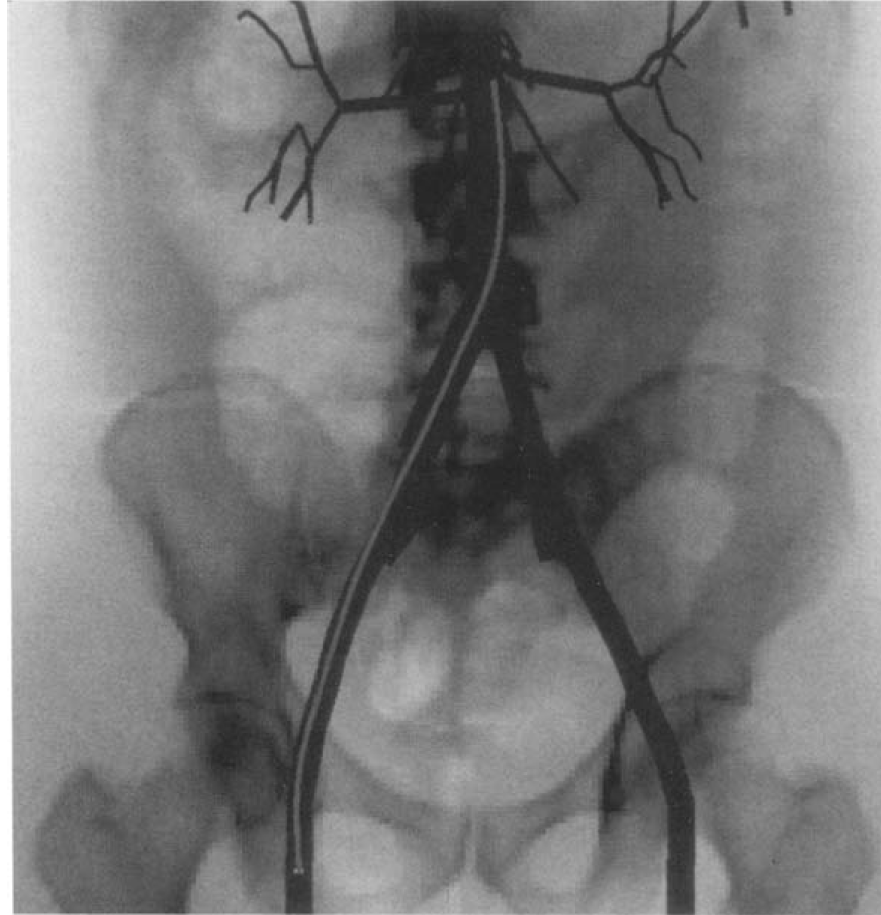
\includegraphics[scale=0.5]{Figures/DaVinci.png}
%\caption{新加坡国立大学和美国约翰·霍普金斯大学医学院共同研究的腹主动脉介入仿真训练系统daVinci\cite{Anderson1998daVinci}}
%\captionof{figure}[腹主动脉介入仿真训练系统daVinci]{新加坡国立大学和美国约翰·霍普金斯大学医学院共同研究的腹主动脉介入仿真训练系统daVinci\cite{Anderson1998daVinci}}
%\label{fig1-1}
%\end{figure}

几乎与此同时,开发daVinci的科研团队在前期工作的基础上,先后实现了用于心血管介入仿真训练的ICard系统(\textbf{\textit{I}}nterventional \textbf{\textit{Card}}iology Simulator)\cite{Wang1997ICard}\cite{Chui1998ICard}\cite{Wang1998ICard}\cite{Cai2004ICard}\cite{Cai2006ICard},
以及用于脑血管介入仿真训练的NeuroCath系统(\textbf{\textit{Neuro}}radiology \textbf{\textit{Cath}}erization Simulator)\cite{Ma2000NeuroCath}\cite{Nowinski2000NeuroCath}\cite{Ma2001NeuroCath}\cite{Li2001NeuroCath}\cite{Nowinski2001NeuroCath}\cite{Anderson2001NeuroCath}\cite{Chui2002NeuroCath}\cite{Anderson2002NeuroCath}\cite{Ma2004NeuroCath}\cite{Volkau2005Vessel}\cite{Ma2005NeuroCath}\cite{Ma2006NeuroCath}\cite{Ma2006aNeuroCath}\cite{Ma2007NeuroCath}。

ICard系统的应用目的是为医学院学生和医生提供一个能够方便地温习心血管介入疗法的平台,同时还希望兼顾评价使用者的技能水平。
该系统的软件部分提供了血管的立体模型和X光效果的显示\cite{Wang1998ICard}\cite{Wang1998aICard}。
血管的影像数据主要来源于VHP。
对于手术涉及的主干血管,限于当时计算机的处理能力,研究团队使用Adobe Systems公司的Photoshop从每张横切影像中将感兴趣的区域中的血管影像的围线标出,然后再计算血管的中心线,最后结合中心线上各点的坐标和相应的半径,得到血管的模型\cite{Wang1998ICard}。
对于病灶涉及的冠状动脉,由于尸体的血管内并没有血液流动以及因此产生的压力,因此这部分较细的血管就会因为其周围肌肉组织的挤压而导致严重变形,这也就造成VHP数据中,冠状动脉的数据几乎全部被破坏\cite{Wang1998ICard}。
为了解决这个问题,该团队的研究人员利用三次元量床(\textbf{\textit{C}}oordinate \textbf{\textit{M}}easuring \textbf{\textit{M}}achine,CMM)\cite{CMMweb}来扫描冠状动脉的钢质模型\cite{KyotoModelweb},从而获得包括完整冠状动脉分支的仿真血管网络,再经过后期的细部处理,得到满足系统要求的冠状动脉血管模型\cite{Wang1998ICard}。
此外,ICard系统还提供了人体的脑血管模型\cite{Serra1997Vessel}\cite{Poston1995Vessel},而脑部影像数据是一组核磁共振血管影像\cite{Wang1998ICard}。
然后,他们通过配准将上述的心脑血管模型与VHP中的主干血管模型连接在VHP数据构建的解剖环境中来获得完整的血管模型\cite{Wang1998ICard}。
至于导管的建模,该系统同样采用了有限元方法\cite{Wang1998ICard}。
ICard提供了两种不同的交互方式:一种是计算机界面,另一种是物理装置界面\cite{Wang1998ICard}。
前者通过点击图形界面上的按钮;后者则通过专门设计的物理装置(导管移动传感装置,\textbf{\textit{C}}atheter \textbf{\textit{M}}ovement \textbf{\textit{S}}ensor device, CMS)\cite{Lim1998ICard}\cite{Lim1997ICard}。
ICard的软件系统所支持的功能包括X光影像显示、立体影像显示与横切面显示、生物医学信号模拟、球囊与支架的植入、以及诸如造影剂的注射等\cite{Wang1998ICard}。

NeuroCath用于仿真球囊和支架的安置、动脉瘤弹簧圈栓塞术(Aneurysm Coiling)等脑血管介入手术。
它继承了前两个系统的许多成熟技术和特性,包括:基于有限元方法的导丝建模以及导丝与血管壁相互作用建模\cite{Wang1996daVinci}\cite{Chui1996daVinci}、基于多模态影像的血管中心线提取\cite{Wang1998ICard}、以及X光效果的显示\cite{Wang1998aICard}\cite{Wang1998ICard}等。
在此基础上,该系统为使用者提供了尽可能丰富和接近真实的体验。如:造影剂注入后在血管内扩散现象、虚拟病人在虚拟手术过程中的生理表征等。
为获得NeuroCath系统所需的脑血管模型,
Cai等人\cite{Ye2002Vessel}\cite{Cai2003aVessel}\cite{Cai2003Vessel}采用了一种利用扫描和混合操作以生成血管段和分岔的结构性方法,该方法提高了血管分岔处的光滑度;
Volkau等人\cite{Volkau2005Vessel}\cite{Volkau2008Vessel}在此基础上提出了基于血管中心线的重建方法,该方法首先提高了血管中心线的光滑程度;其次抑制了在分割和骨架化过程中引入的噪声,从而提高了(重建血管时所依赖的)血管半径的精确度。
NeuroCath的操作风格与ICard类似,也提供了可视界面交互和物理交互装置交互两种方式\cite{Nowinski2001NeuroCath}。
其中,研究人员为NeuroCath专门设计了物理交互装置 --- TiC(\textbf{\textit{T}}actile and \textbf{\textit{i}}mage \textbf{\textit{C}}ontrol)\cite{Chui1999TiC}\cite{Ma1999TiC},它由触觉子系统和影像操作子系统等两个主要部分组成。
前者可以使操作者能够操作导管和导丝进行与真实血管介入手术中类似的运动;后者则通过一台虚拟工作站来操作可视界面中提供的X光影像的视角。
此外,NeuroCath还能为使用者提供血管内的视角,该功能用于血管内窥镜导航的仿真\cite{Nowinski2001NeuroCath}。
NeuroCath最初在约翰-霍普金斯大学医学院进行了验证,随后还获得了包括德国萨尔大学诊断介入神经放射学诊所、中国北京宣武医院、以及德国国立信息技术研究中心等医院和研究机构的验证许可,并收到了比较满意的反馈\cite{Ma2007NeuroCath}。

为了提高工作效率,科研团队还开发了若干CAD软件,它们分别用于导管等血管介入器械,如:CathWorks\cite{Cai1998CathWorks}\cite{Cai2000CathWorks}、DCSM\cite{Li2001DCSM}等; 以及血管等人体器官的建模的CAD软件工具,如:VasWorks\cite{Cai2003Vessel}、Vascular Editor\cite{Ma2007NeuroCath}等。

近几年,该团队仍有部分研究人员致力于心血管介入手术仿真的研究,重点是心脏建模\cite{Chiang2011}\cite{Chiang2012}等。

位于美国麻省的三菱电气实验室(Mitsubishi Electric Research Laboratories,MERL)\cite{merlweb}和美国创新微创疗法中心(Center for Innovative Minimally Invasive Therapy,CIMIT)\cite{cimitweb}联合发起了ICTS项目\cite{Dawson2000ICTS}\cite{Cotin2000ICTS}\cite{Shaffer1999ICTS}。
ICTS的全称是“Interventional Cardiology Training System”(介入心脏病学训练系统),该系统旨在为学习者提供训练平台,并为引入新的医学器材和手术方法提供展示平台\cite{Cotin2000ICTS}。
ICTS实现了X光效果的解剖环境、建立了导管的物理模型和血液流动模型、并制作了触觉接口装置\cite{Cotin2000ICTS}。
此外,该系统还实现了一种手术学习机制“Virtual Rounds”\cite{Shaffer1999ICTS},该学习机制复现了心血管介入手术的基本步骤,为使用者的训练评估提供了基础。
文献\cite{Dawson2000ICTS}中提到,ICTS系统当时正准备在欧洲投入其首次训练试验。

然而,当时的ICTS仅仅处于样机验证阶段,根据与比利时Guidant公司的合同,该项目后来被移交至英国Virtual Presence公司以完成系统的研发,并最终由瑞典Mentce公司\cite{menticeweb}将其商业化\cite{GuidantMenticeNewsWeb}\cite{coles2011surveyCRaIVE},这就是该公司的VIST系列产品。
目前,VIST系列的两种仿真平台已经能够仿真的血管介入技术有:冠状动脉造影、心脏节律管理、跨室间隔穿刺、肾动脉介入、髂内动脉介入、膝关节以下血管介入、主动脉内窥修复、颈动脉介入、脑血管介入、子宫动脉栓塞术等\cite{menticeweb}。
其中已经获得医学验证的技术有:颈动脉介入手术的仿真训练\cite{Dayal2004VIST}\cite{Hsu2004VIST}\cite{Nicholson2006VIST}\cite{Patel2006VIST}\cite{Cates2007VIST}\cite{VanHerzeele2009VIST},肾动脉介入术\cite{Aggarwal2006}\cite{Glaiberman2008VIST},髂内动脉介入术\cite{Chaer2006VIST}\cite{Berry2007VIST}\cite{VanHerzeele2008VIST},冠状动脉介入术\cite{Gallagher2006VIST}等。

CIMIT的Sim小组\cite{medicalsimweb}和法国INRIA的Shacra团队\cite{shacraweb}联合开发的EVE项目\cite{Wu2005EVE}是一种用于仿真脑血管介入手术的系统。
它提供了适用于复杂血管系统内部的具有实时的碰撞检测和碰撞响应性能的导管有限元模型\cite{dequidt2007EVE}\cite{Duriez2006EVE}\cite{Lenoir2006EVE}\cite{Lenoir2005EVE}\cite{Cotin2005EVE},
具有X光显示效果的头颈部解剖模型\cite{Wu2011EVE}\cite{Luboz2005EVE}\cite{Muniyandi2003EVE},
以及血流动力学模型、虚拟造影剂、心脏搏动和呼吸\cite{Wu2007EVE}等视觉效果。
文献\cite{Dequidt2008EVE}介绍了该团队进行动脉栓塞术中弹簧圈的仿真以及验证的情况。
操作装置方面,研究人员设计了专用的触觉接口装置ABEL和专用的径向跟踪装置Cain\cite{medicalsimweb}。

此外,Shacra团队在EVE等项目的工作基础上,开发并维护着一个专门用于医学仿真的工具库 --- SOFA(\textbf{\textit{S}}imulation \textbf{\textit{O}}pen \textbf{\textit{F}}ramework \textbf{\textit{A}}rchitecture)\cite{Allard2007SOFA}。

意大利CRS4小组发起了ViVa项目(\textbf{\textit{Vi}}rtual \textbf{\textit{Va}}scular project)\cite{abdoulaev1998},该项目的研究目标是为现代血流动力学研究者和心脏内科医生提供一系列的工具,帮助他们分析和解释在研究和临床过程中遇到的不断增多的相关信息。
这些工具包括:图像处理与分割、实时立体体数据可视化、立体几何重建、立体网格生成、以及血流仿真和可视化等。
在此基础上,Gobbetti等人\cite{Gobbetti1998}研究并实现了用于仿真血管镜的系统。
该系统以从标准医学影像模态所获取的数据作为输入,将其当作可供交互的虚拟环境;系统支持立体直接体绘制的实时导航和动态内窥镜的控制,可交互的组织分类,以及为实现形态学特性测量而摘取可交互点等。
Zorcolo与Gobbetti等人\cite{Zorcolo1999}\cite{Gobbetti2000}\cite{Zorcolo2000}开发了一种实验性的导管插入系统。
该系统支持头部跟踪的立体视感,该视感通过从不同视角观察体重建而产生,体重建则与直接的立体触觉交互相匹配,这属于增强现实系统的范畴。

英国的CRaIVE(\textbf{\textit{C}}ollaborators in \textbf{\textit{R}}adiological \textbf{\textit{I}}nterventional \textbf{\textit{V}}irtual \textbf{\textit{E}}nvironments)\cite{CRaIVEweb}进行了与介入手术的仿真训练相关的研究。
他们的研究主要集中于血管介入手术中血管系统的分割与重建\cite{Luboz2008aCRaIVE},
血管和导管及其相互作用的建模和验证\cite{Luboz2010CRaIVE}\cite{Luboz2009aCRaIVE}\cite{Luboz2008CRaIVE},
Seldinger穿刺术的仿真\cite{luboz2009CRaIVE}\cite{John2008CRaIVE},
以及穿刺术之前的腹股沟触诊的仿真\cite{Coles2011CRaIVE}\cite{Coles2009CRaIVE}。
此外,文献\cite{Coles2010CRaIVE}还对若干应用于穿刺仿真中的触觉反馈装置的性能进行了测试和比较。

法国巴黎第十二大学计算机工程与自动化实验室进行了基于虚拟现实技术的腹主动脉介入手术仿真系统的研究\cite{Ghembaza2004Paris12U}。
系统中,腹主动脉和导管的物理模型采用基于位移的有限元方法来建立;为了实现连续的碰撞响应,研究人员采用了基于Cubic Spline的参数估计方法。

由荷兰列文胡克癌症研究所和乌德勒支大学图像科学研究所发起的MIVIS项目(\textbf{\textit{M}}inimally-\textbf{\textit{I}}nvasive \textbf{\textit{V}}ascular \textbf{\textit{I}}ntervention \textbf{\textit{S}}imulation)\cite{alderliesten2002NKI}\cite{Konings2003NKI}\cite{alderliesten2004NKI}\cite{Bosman2005NKI}\cite{alderliesten2007NKI}\cite{alderliesten2007aNKI}
主要进行了腹主动脉导管介入的仿真,对导管在血管内的运动仿真是该项目的研究重点。
血管的几何建模采用了Fuzzy Connectedness算法\cite{Udupa1996NKI}\cite{alderliesten2002NKI}\cite{alderliesten2004NKI};
而其物理建模则利用胡克定律来模拟血管壁的组织特性\cite{alderliesten2002NKI}\cite{alderliesten2004NKI};
导管模型的物理特性则建立在准静态力学(quasi-static mechanics)的基础上\cite{alderliesten2002NKI}\cite{alderliesten2004NKI};
并在此基础上进行了实物对比验证\cite{alderliesten2002NKI}\cite{alderliesten2004NKI}。
Konings等人\cite{Konings2003NKI}提出了一种用于导管在血管内运动仿真的半解析算法,并进行了导管在平面弯道内运动仿真性能的验证分析。
Bosman等人\cite{Bosman2005NKI}研究了利用一种进化算法以替代面向特定问题的一阶解析估计算法,从而解决仿真过程中的优化问题的优劣,并证明采用前者更有利于系统性能的优化。
Alderliesten等人\cite{alderliesten2007NKI}又在此基础上进一步拓展了算法性能对比的研究,并证明采用共轭梯度算法或者进化算法能够在仅产生轻度误差的前提下,显著地减少计算时间。
文献\cite{alderliesten2007aNKI}中报告了该项目中的导丝模型已经能够仿真导丝与血管壁之间的摩擦。

德国曼海姆大学、海德堡大学与德国维尔茨堡大学医院联合研究的CathI(\textbf{\textit{Cath}}eter \textbf{\textit{I}}nstruction System)用于血管介入尤其是经皮腔内冠状动脉成形术(\textbf{\textit{P}}ercutaneous \textbf{\textit{T}}ransluminal \textbf{\textit{C}}oronary \textbf{\textit{A}}ngioplasty,PTCA)的仿真\cite{rebholz2004cathi}\cite{Hoefer2002CathI}。
该系统提供了一系列的功能设施用于实现尽可能真实的血管介入手术仿真训练\cite{rebholz2004cathi},包括:个人档案、不同型号的血管介入器械(导管、导丝、球囊和支架等)、控制C型臂的脚踏板、控制射线开关和造影剂剂量的设定、限制照射时间和介入手术总时间的设定以及人体生理指标的设定等。
该系统的数据来自真实病例的术中X光造影,影像中能够观察到真实病例所具有的典型特征;而所选取的影像包含了一个心动周期的关键帧,因而能够提供准确的心脏搏动,这样可以为受训者提供最真实的视觉效果。
血管被抽象为刚体且横截面为圆\cite{Hoefer2002CathI}。
导管则被抽象为一列刚性的圆柱体,当导管与血管壁发生交互时,由这个几何模型确定其与血管壁的接触点,在此基础上计算应该发生的弯曲等形变,但未考虑导管与血管壁之间的摩擦\cite{rebholz2004cathi}。
在操作装置上,系统采用了导管室所使用的原始机构,最大限度地模仿真实的导管术操作工具;而测量导丝进给的功能实现上,则通过反射自附着在导丝上的玻璃纤维的光线的变化来测量导丝的运动,这种方法克服了传统机械方式所具有的摩擦和滑动等不足\cite{Hoefer2002CathI}。
此外,系统提供的个人档案功能能够记录受训者在仿真训练过程中的一些必要的信息,并且能够导出为Excel文件,但并未实现自动的评价功能\cite{rebholz2004cathi}。

德国达姆施塔特科技大学和德国维尔茨堡大学医院进行了基于计算机仿真的冠状动脉造影中针对病例的导管最优选择方面的研究\cite{Rahman2012Darmstadt}\cite{Rahman2011bDarmstadt}\cite{Rahman2011aDarmstadt}\cite{Flehmann2011Darmstadt}。
工作的第一步是计算病例影像中主动脉的几何参数,一种新的分割后的融合方法被用于主动脉的几何模型的获取\cite{Flehmann2011Darmstadt}。
在此基础上,文献\cite{Rahman2011bDarmstadt}和\cite{Rahman2011aDarmstadt}分别介绍了基于计算机仿真的左右两侧冠状动脉造影中针对病例的导管最优选择方法。
根据这两篇文献的结论,医师应能够更通过这些方法获得相应侧的冠状动脉介入时所需导管的最佳选择方案。
文献\cite{Rahman2012Darmstadt}介绍了导管模型的建模方法,各种型号的导管的物理特性通过FEM方法进行建模,其具体工作使用了SOFA\cite{Allard2007SOFA}。

意大利莱切大学创新工程部的研究人员进行了心血管介入支架置入术仿真的研究\cite{aloisio2006HERMES}\cite{aloisio2006aHERMES}\cite{aloisio2005HERMES}\cite{aloisio2004HERMES}。
其中的部分成果借鉴了由意大利CETMA集团发起的HERMES项目(\textbf{\textit{HE}}matology \textbf{\textit{R}}esearch virtual \textbf{\textit{ME}}dical \textbf{\textit{S}}ystem,用于血液学研究的虚拟医学系统)\cite{aloisio2005HERMES}。
为了获得血管的准确形变,该系统采用有限元方法建立血管系统的模型\cite{aloisio2004HERMES}。
系统的操作装置能够再现支架置入过程中,手术工具发生的形变\cite{aloisio2005HERMES}。
不同于其它仿真系统的是,本系统还能够支持病例模型数据的网络检索和获取功能\cite{aloisio2006aHERMES}\cite{aloisio2006HERMES}。
受训者可以利用这个功能,从支持相关数据共享的医疗机构获取需要的病例影像数据,这为病例数据的获取提供了极大便利,使受训者能够方便地接触到更丰富的病例。

瑞士洛桑联邦理工学院机器人系统实验室设计并实现了一种用于仿真脑血管介入手术的系统\cite{Wang2007EPFL}\cite{Ilic2005EPFL}\cite{Moix2005EPFL}\cite{Ilic2005aEPFL}\cite{Ilic2005bEPFL}。
该系统的研究工作提出了一种基于物理特性的线形模型,以及一种快速碰撞检测策略\cite{Wang2007EPFL}。
前者所体现的仿真物理特性模拟了导丝的弹性特征,后者可以提供连续的碰撞检测,这与中心线方法相比,能够揭露出血管壁表面的更多细节。
同样地,该系统也提供了X光显示效果的解剖环境。
此外,该实验室还设计并实现了用于脑血管介入手术仿真的4自由度触觉接口装置\cite{Ilic2005EPFL}\cite{Moix2005EPFL}\cite{Ilic2005aEPFL}。
通过实验测量了血管介入手术中,血管因球囊膨胀过程中的弹性模量\cite{Ilic2005bEPFL}。
根据文献\cite{Wang2007EPFL},接下来的工作将是计算机仿真部分与触觉接口装置的整合。

日本名古屋大学的研究人员进行了用于分布式血管内遥操作手术的虚拟环境研究\cite{Arai1994Nagoya}\cite{Arai1995Nagoya}\cite{Arai1996Nagoya}。
该虚拟环境主要为远离手术现场的医生提供直观的视觉和触觉。为此,该虚拟环境提供了三维显示功能和专门设计的操作机构。
显示功能中的血管和导管的建模都比较简化:导管模型以常数曲率弯曲、血管模型则被抽象为不同半径的圆柱体\cite{Arai1994Nagoya}\cite{Arai1995Nagoya}。
该分布式遥操作手术系统用于脑血管介入手术,研究人员在东京市(早稻田大学)与名古屋市(名古屋大学)之间(距离350km)进行了实验。
整个过程中的数据通过异步传输模式的光纤传输\cite{Arai1996Nagoya}。

日本名古屋大学微纳米系统工程系以及藤田保健卫生大学和安城厚生病院的研究人员进行了脑血管介入手术仿真的研究\cite{Ikeda2004Nagoya}\cite{Ikeda2005Nagoya}\cite{Ikeda2005aNagoya}\cite{Ikeda2006Nagoya}\cite{Ikeda2007Nagoya}。
与其他研究项目的思路不同,该项目的研究人员仍然坚持实物仿真训练,利用硅胶等材料、通过精密的加工工艺以人体头部CTA和MRA影像为依据,制作高精确度(解析度达到亚毫米级别)的人体脑血管的物理模型,为脑血管介入手术的训练提供操作场景\cite{Ikeda2005Nagoya}。
这种物理模型能够再现血管的物理特性,以及导管与其内壁发生的摩擦。

日本理化学研究所等科研机构开展了用于血管介入手术仿真的研究\cite{takashima2009RIKEN}\cite{takashima2007RIKEN}。
导丝被抽象为若干段粘弹性弹簧(viscoelastic spring),其近端由于受限于导丝模型,故被抽象为刚性管道,而血管则被抽象为横截面为圆的弹性圆柱体\cite{takashima2009RIKEN}。
血管的几何模型通过“分割血管-提取中心线-根据半径重建血管”的方式获得\cite{takashima2009RIKEN}。
为了获得准确的、对导丝与血管壁之间相互作用的仿真效果,文献\cite{takashima2007RIKEN}采取了实物试验与计算仿真相互比较的方法对这一场景下的摩擦和接触进行了实验和数值分析,从而得出仿真系统中准确的血管模型参数的重要性。

日本香川大学工学部的郭书祥等人研究并实现了用于脑血管介入手术仿真的系统\cite{Gao2012aGUO}\cite{Gao2012bGUO}\cite{Gao2012cGUO}。
该系统由为使用者提供视觉感受的虚拟现实软件和为使用者提供触觉感受的导管操作装置组成\cite{Gao2012aGUO}。
在脑血管模型的获取过程中,研究人员通过若干开源工具,对血管影像进行阈值处理,手动记录血管的中心线坐标,使用一种被称为“四邻域法”的方法寻找血管的边缘像素点,在此基础上重建血管的几何模型\cite{Gao2012bGUO}。
导管模型的建立则采用了有限元的方法\cite{Gao2012cGUO}。

美国HT Medical公司开发的CathSim系统用于仿真外周静脉内导管术\cite{ursino1999cathsim},以及护士技术中的静脉穿刺\cite{Barker1999CathSim}。

美国乔治·华盛顿大学研究了用于下腔静脉滤器置入的虚拟训练系统\cite{Hahn1998GWU},该仿真系统提供下腔静脉滤器置入术的教学和测试。
为了获得X光的视觉效果,研究人员采用了一种“伪体绘制”的渲染方法\cite{Park1996GWU},该方法能够生成影像数据的$360^\circ$的视觉效果,并且支持虚拟场景中摄像头沿虚拟人体的径向移动。
造影剂则被建模成粒子系统,该粒子系统由导管的尖端触发,系统则在不同的时刻进行记录其向心脏一侧运动过程中的位置\cite{Hahn1998GWU}。
此外,该系统还能够模拟导管与血管壁之间的摩擦\cite{Hahn1998GWU}。

加拿大的CAE公司\cite{caeweb}开发了一种用于心血管介入的仿真训练系统CathLabVR。
该系统能够进行冠状动脉经皮介入、外周动脉经皮介入、以及心脏外科手术等的仿真训练。
以色列的Simbionix公司\cite{simbionixweb}研发了一种用于血管介入的仿真训练系统Angio Mentor。
该系统能够进行介入式心脏治疗、介入式放射学诊断、血管手术、心脏手术、电生理学、介入式脑血管治疗、以及胸腔外科手术等的仿真训练。
文献\cite{hislop2009Simbionix}\cite{Lee2012Simbionix}报告了该系统在实际使用情况。
文献\cite{Petri2013Comparison}对主要的产品级别的仿真系统进行了临床验证。

美国的Medical Simulation公司开发了SimSuite\cite{simsuiteweb}系列血管介入手术仿真系统。
该系列中的Compass系统是一种便携式的仿真系统,这种系统为医师提供了随时进行进行基本流程的训练的条件。
该系列中的Infinity系统是一种能够运行在iPad等平板电脑上的仿真应用。
该系列中的Simantha系统是SimSuite的重量级系统,它能够支持心血管介入、脑血管介入、以及外周动脉介入等疗法的虚拟仿真。此外,该系统还支持用户建立自定义的训练课程。
文献\cite{Dawson2007SimSuite}介绍了该系统的临床验证效果。

\subsection{国内研究现状}
\label{sec1-4-2}

近年来,随着我国社会经济的不断发展,国民生活水平也有了长足的提高,人们一方面享受到了较
好的物质条件带来的多方面的益处,一方面也由于缺乏端正的健康生活意识而出现了各种由于膳食
结构不合理、体力消耗水平过低而引起的疾病,其中以冠心病等心脑血管疾病为代表的人体循环系
统疾病的发病率和致死率呈逐年上升趋势,这一趋势已引起了医学界和公共卫生部门的高度重视。
正是这样,国内高校和科研院所近年开展与临床手术应用相关的生物工程项目不断增多。然而,由
于我国在相关方面的科研基础与发达国家存在差距,再加上我们在科研成果转化为实际应用方面的
滞后,目前,国内虚拟手术训练的研究仍处于初级阶段。

香港中文大学的计算机科学与工程系开展了血管介入手术仿真的研究\cite{guo2007CUHK}\cite{Chui2010CUHK}\cite{Li2011CUHK}\cite{Li2012CUHK},并成为2009年该校举行50周年校庆时的重大成果之一\cite{cuhkweb}。
该系统的血管和导管的集合模型的建立,利用了中心线提取、图重建、曲线拟合、以及曲线帧技术;为了给形变模型赋予非线性的生物力学特性,采用了基于物理处理单元(Physics Processing Unit,PPU)的增量式Voigt模型\cite{guo2007CUHK}。
该系统通过一种非牛顿流的光滑粒子流体动力学(Smoothed Particle Hydrodynamics,SPH)形式来模拟血液在血管内的流变;
通过流体结构相互作用的一种纯拉格朗日粒子形式来模拟血液与血管的相互作用,其中,血管壁结构被抽象为虚拟粒子;
并在此基础上,模拟了血栓形成与消溶的过程\cite{Chui2010CUHK}。
导管与血管之间相互作用的模拟则基于最小总势能的原理,其中的势能是导管弯曲时的弹性势能、血管壁变形时的势能,以及外力所做功的总和;
导管形变的模拟则利用了有限元的方法\cite{Li2011CUHK}。
此后,研究人员还研究了一种快速稳定的多网格求解器,以保证仿真的真实性和实时性\cite{Li2012CUHK}。

中国科学院深圳先进技术研究院的马炘等人\cite{Ma2010SIAT}\cite{Ma2010aSIAT}进行了脑血管介入手术仿真系统的研究。
该系统的脑血管建模,吴剑煌等人采用了面向三角网格的自适应细分模式\cite{Wu2006SIAT},所得血管模型的数据量得到了合理地精简,提高了血管模型在使用中的渲染速度和碰撞检测速度。
导管等医疗器械的建模采用了有限元方法。导管被抽象为由许多节点相连的定长线段,对各个节点赋予物理属性,这样节点与节点就成了机构学上的铰接结构,当受到外力时,节点处可以自由旋转\cite{Ma2010SIAT}。
对导管与血管壁的相互作用的仿真,该系统的碰撞检测分为初步检测、精确检测、和确定碰撞位置等三个步骤\cite{Ma2010SIAT}。
该系统还实现了触力反馈,并设计和实现触觉反馈装置\cite{Ma2010SIAT}。

国防科技大学的熊岳山等人对虚拟心脏介入手术的相关方面进行了研究,如:
几何模型构建技术\cite{han2005master}、
血流模拟和特效场景\cite{ren2005master}\cite{Ren2006NUDT}、
弹簧-振子模型\cite{wang2006master}\cite{Wang2008NUDT}、
医疗器械的三维建模\cite{zhu2007master}
以及碰撞检测技术\cite{kang2007master}等,
最近,该系统已经初步实现,文献\cite{Tan2012NUDT}报告了该工作的最新进展。
其中,心脏模型的构建利用了Delaunay三角化方法,血管建模则采用了NURBS曲面;
通过组合弹簧振子联动模型的方法仿真了心脏搏动\cite{Wang2008NUDT};
采用风腔结构\cite{Ren2006NUDT}模拟冠状动脉和主动脉,提高了血流仿真效果。
此外,该系统还实现了虚拟造影剂、X光显示效果、以及导管等柔性器械的建模\cite{Tan2012NUDT}。

其中与本课题研究方向有一定关系的有:
天津大学的冯鹰\cite{li2005master}等人于2005年设计并实现了用于腹腔镜手术的虚拟训练系统;
该校的王树新等人\cite{zeng2006master}于2006年研究了面向显微外科手术的虚拟血管缝合仿真系统。
上海交通大学的顾力栩等人开展了虚拟手术系统中模拟手术场景的渲染和平台的创建工作\cite{zheng2008master}以及血管内血流模拟方面的工作\cite{huang2011virtual};
该校的谢叻等人则在虚拟手术的碰撞检测\cite{wu2010virtual}和触力反馈\cite{wu2011virtual}方面进行研究。
复旦大学进行了房间隔缺损介入封堵术的三维可视化模拟\cite{Zhao2006Fudan}。
北京工业大学研究了心血管系统动脉粥样硬化病灶部位的血流动力学\cite{Huang2003BJUT}。

\section{本文布局}
\label{sec1-5}

%本节叙述内容:
%\begin{enumerate}
%  \item 研究工作目的
%  \item 论文内容布局
%  \item 组内相关工作
%\end{enumerate}

本文所述工作的目的是:以真实的心血管微创介入导管术为原型,利用计算机相关学科的知识和
技术,研究并实现一种能够以虚拟现实或增强现实的方式来模拟该原型的手术训练系统。该系统
应当具备友好的图形界面;提供为获得足够真实的感受所需的反馈,包括:视觉方面,足够真实
的,与介入式导管术相关的人体解剖结构,以及在外观和物理特性方面足够真实的手术器械(即
导管);触觉方面,提供与虚拟环境中的视觉反馈相一致的触觉感受,如:导管在进给过程中,
若其顶端触碰到血管壁,操控者手持的触觉接口则会向其提供一个阻力的感受,使操控者仿佛真
实地感受到自己手中操控的导管的顶端碰到了血管的内壁一样。在这样一个过程中,我们所研发
的系统足以为操控者提供一个足够真实具体的手术环境,从而使学员能够获得与其在真实生物体
上进行手术相近的体验,学到远比教科书讲授内容更为真切的技能;使有经验的医师能够在开展
真实手术之前,演练并验证自己的手术方案,提高手术的成功率。

本文开篇介绍本研究项目的基本情况,以及与本研究项目有关的同行的研究进展;
接下来的每章叙述一个导管术训练系统的关键技术环节;最后一章总结我们在研究工作中的成果,
经验,与教训,并展望本项目未来的一些可能的发展动向。全文分为正文和附录等两部分。正文共八章:第一章是全文绪论,
概括介绍本项目的研究动机、研究背景、以及本文的主要内容,详细描述与本文所述工作相关的
典型样机和关键技术在国内外研究情况和发展历史;第二章是医学背景介绍,比较详细地记述了
与本文所述工作相关的医学知识,包括介入心脏病学和医学影像技术等内容;第三章是血管模型的可视化,介
绍了为从CTA中获得血管系统所对应的像素信息所进行的主要工作以及工作成果,详
细描述本环节工作所用到的关键技术内容,以及在此基
础上获得血管系统的可视化模型所进行的主要工作以及工作成果,深入描述了本环节工作所用到
的关键技术内容;第四章是心脏模型的提取与可视化,介绍了基于CTA的心脏模型的分割与可视
化工作和工作成果,描述了本环节工作所用到的关键技术内容;第五章是组织的物理特性建模,
具体介绍了器官组织物理特性的分析与建模过程;第六章是手术过程中特殊动态效果的实现,描
述了为实现诸如虚拟造影剂、可视化模型的X光显示等可视效果而做的工作,展示了工作成果;
第八章是手术流程的状态机模型研究,主要介绍将冠状动脉导管术的流程进行计算机建模的一种
方法;
第八章是总结与展望,客观、全面地总结全文内容,概括本研究项目所取得的工作成果,列出在
此过程中表现出来的一些教训,最后对本研究工作的未来发展做了一些预测。附录共两章,附录A给出了正文中的一些原理的数学推导;附录B记录了笔者在本项目的研究过程中对软件工程的一些思考。
文末附有参考文献和本人在学期间发表文章的清单等。

本文所述工作是“经皮介入冠脉导管术仿真系统的设计与研究”的一部分,工作任务涉及血管系
统和心脏等解剖结构的场景生成和仿真。关于该仿真系统中的手术工具的物理建模与仿真,请参
考组内同事米韶华的博士学位论文《XXX》以及相关的已发表科技文章。

本文所述工作获得了国家自然科学基金(61225017)和北京市优秀博士学位论文指导教师科技项
目(YB20108000103)资助。在此,笔者谨向国家自然科学基金委员会和北
京市教育委员会表示由衷的感谢! 